\pdfminorversion=4
\documentclass[aspectratio=169]{beamer}

\mode<presentation>
{
  \usetheme{default}
  \usecolortheme{default}
  \usefonttheme{default}
  \setbeamertemplate{navigation symbols}{}
  \setbeamertemplate{caption}[numbered]
  \setbeamertemplate{footline}[frame number]  % or "page number"
  \setbeamercolor{frametitle}{fg=white}
  \setbeamercolor{footline}{fg=black}
} 

\usepackage[english]{babel}
\usepackage{inputenc}
\usepackage{tikz}
\usepackage{courier}
\usepackage{array}
\usepackage{bold-extra}
\usepackage{minted}
\usepackage[thicklines]{cancel}
\usepackage{fancyvrb}

\xdefinecolor{ucred}{rgb}{0.50,0,0}
\xdefinecolor{dianablue}{rgb}{0.18,0.24,0.31}
\xdefinecolor{darkblue}{rgb}{0.1,0.1,0.7}
\xdefinecolor{darkgreen}{rgb}{0,0.5,0}
\xdefinecolor{darkgrey}{rgb}{0.35,0.35,0.35}
\xdefinecolor{darkorange}{rgb}{0.8,0.5,0}
\xdefinecolor{darkred}{rgb}{0.7,0,0}
\definecolor{darkgreen}{rgb}{0,0.6,0}
\definecolor{mauve}{rgb}{0.58,0,0.82}

\title[2026-07-15-scipy-oaec-gullymap]{\textcolor{black}{From LiDAR to action: detecting upland gullies to combat erosion and forest fires}}
\author{Jim Pivarski}
\institute{University of Chicago -- Data Science Institute}
\date{July 15, 2026}

\usetikzlibrary{shapes.callouts}

\begin{document}

\logo{\pgfputat{\pgfxy(0.11, 7.4)}{\pgfbox[right,base]{\tikz{\filldraw[fill=ucred, draw=none] (0 cm, 0 cm) rectangle (50 cm, 1 cm);}\mbox{\hspace{-8 cm}
\includegraphics[height=1 cm]{uchicago-logo-long.png}\hspace{0.1 cm}{
\includegraphics[height=1 cm]{dsi-logo-long.png}}\hspace{0.1 cm}}}}}

\begin{frame}
  \titlepage
\end{frame}

\logo{\pgfputat{\pgfxy(0.11, 7.4)}{\pgfbox[right,base]{\tikz{\filldraw[fill=ucred, draw=none] (0 cm, 0 cm) rectangle (50 cm, 1 cm);}\mbox{\hspace{-8 cm}
\includegraphics[height=1 cm]{uchicago-logo.png}{
\includegraphics[height=1 cm]{dsi-logo.png}}\hspace{0.1 cm}}}}}

% Uncomment these lines for an automatically generated outline.
%\begin{frame}{Outline}
%  \tableofcontents
%\end{frame}

% START START START START START START START START START START START START START

\begin{frame}{Fuels to Flows: solving two problems at once}
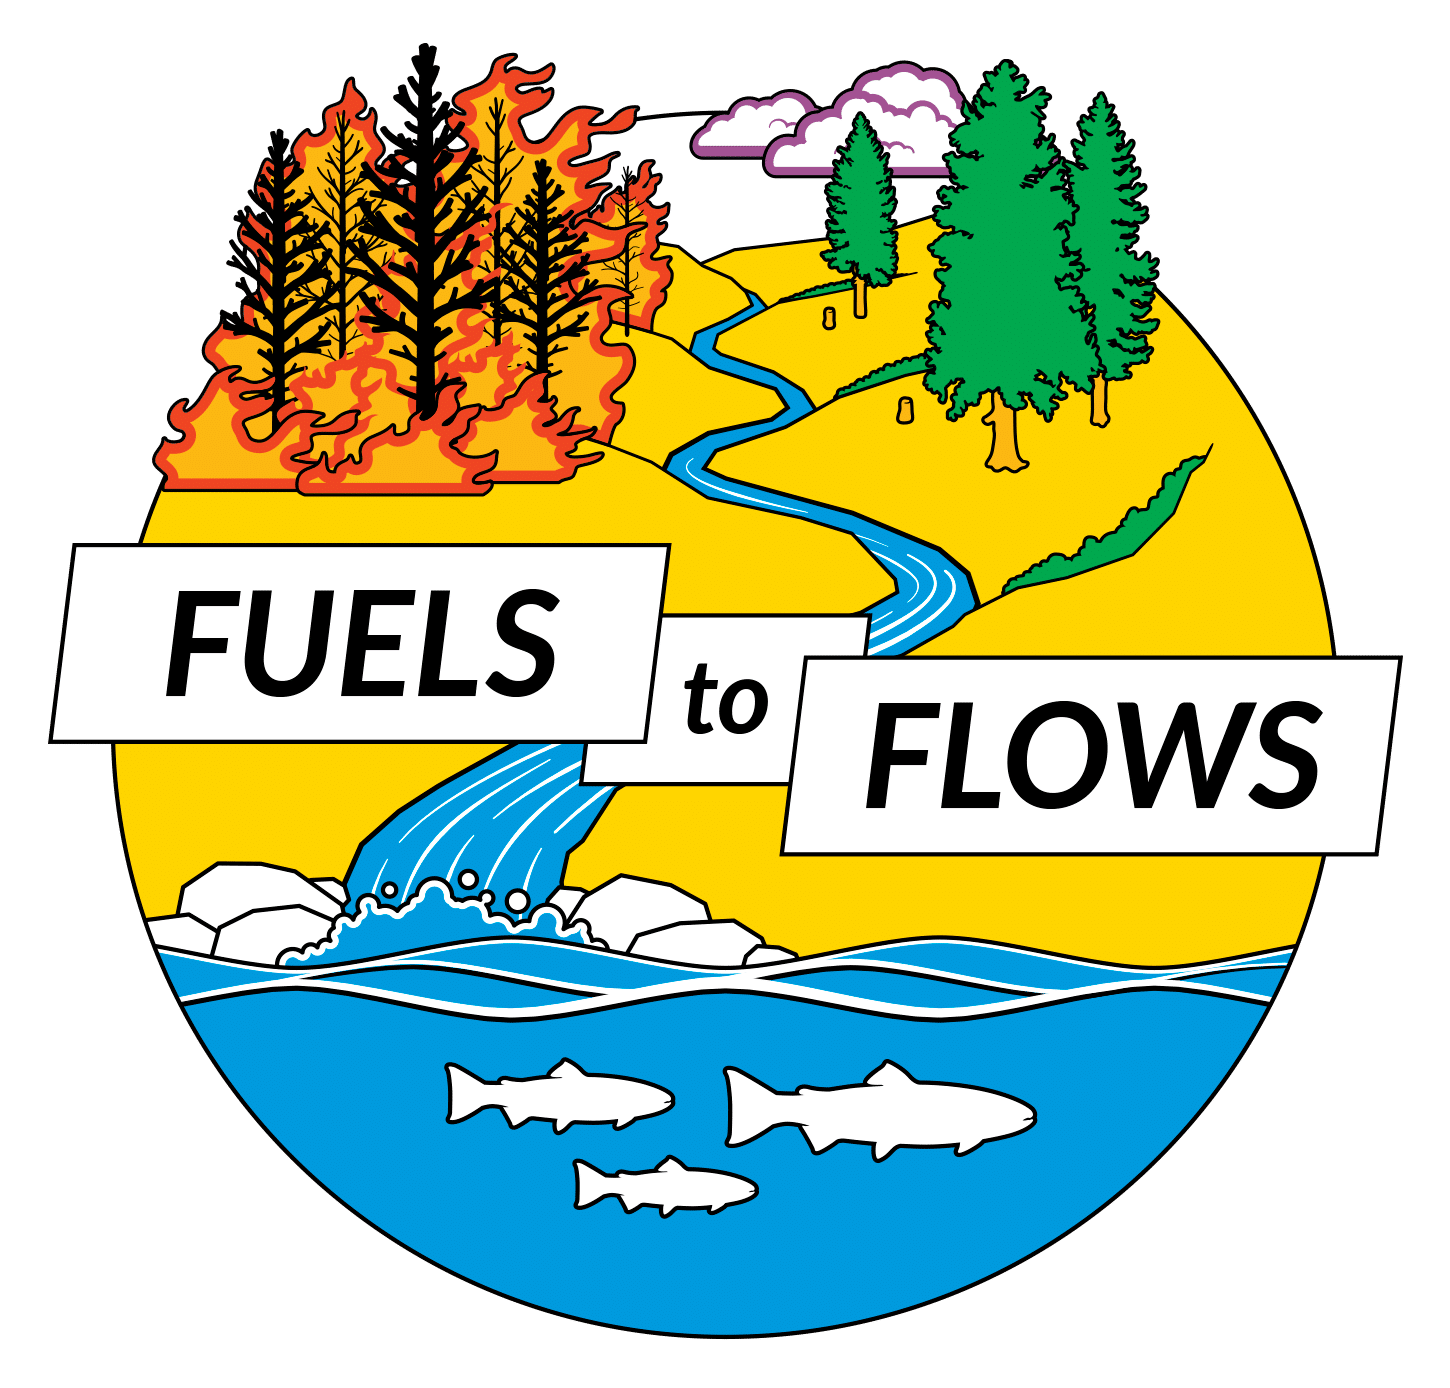
\includegraphics[width=0.1\linewidth]{img/fuels-to-flows-logo.png}
\begin{columns}
\column{0.2\linewidth}
\textcolor{blue}{Removing ladder fuels that cause forest fires.}
\column{0.6\linewidth}
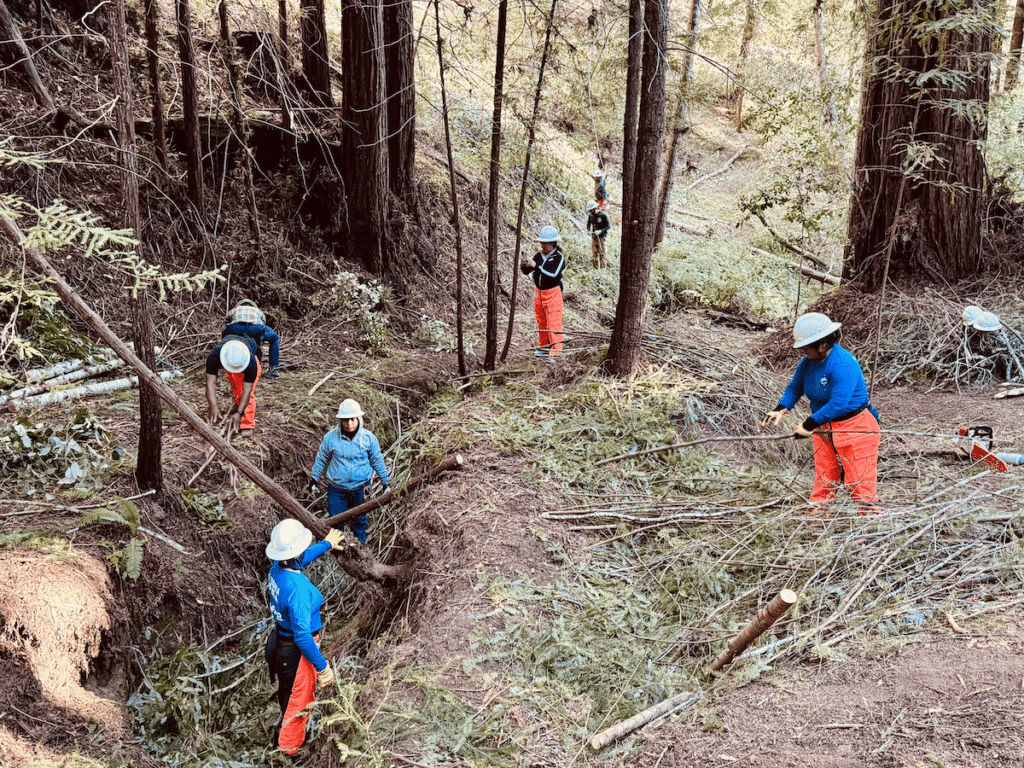
\includegraphics[width=\linewidth]{img/fuels-to-flows1.png}
\column{0.2\linewidth}
\textcolor{blue}{Stuffing gullies to decrease erosion.}
\end{columns}
\end{frame}

\begin{frame}{Fuels to Flows: solving two problems at once}
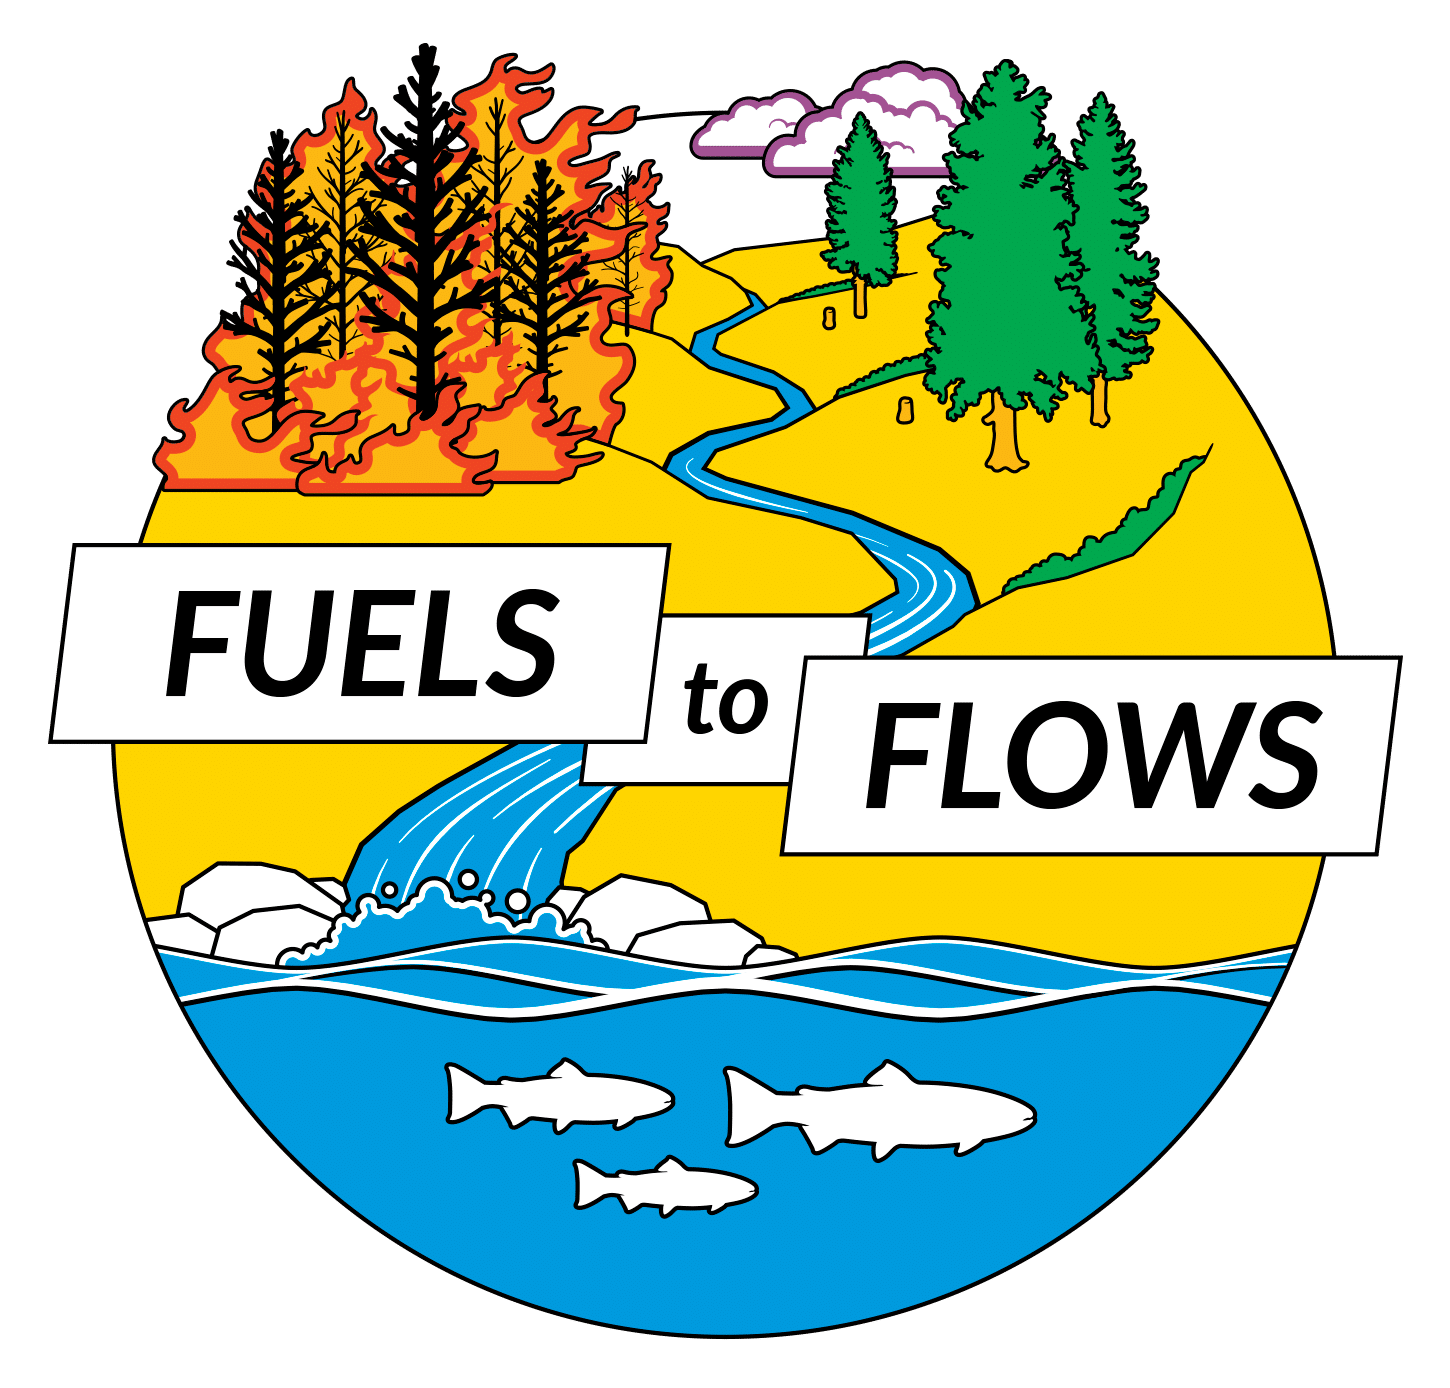
\includegraphics[width=0.1\linewidth]{img/fuels-to-flows-logo.png}
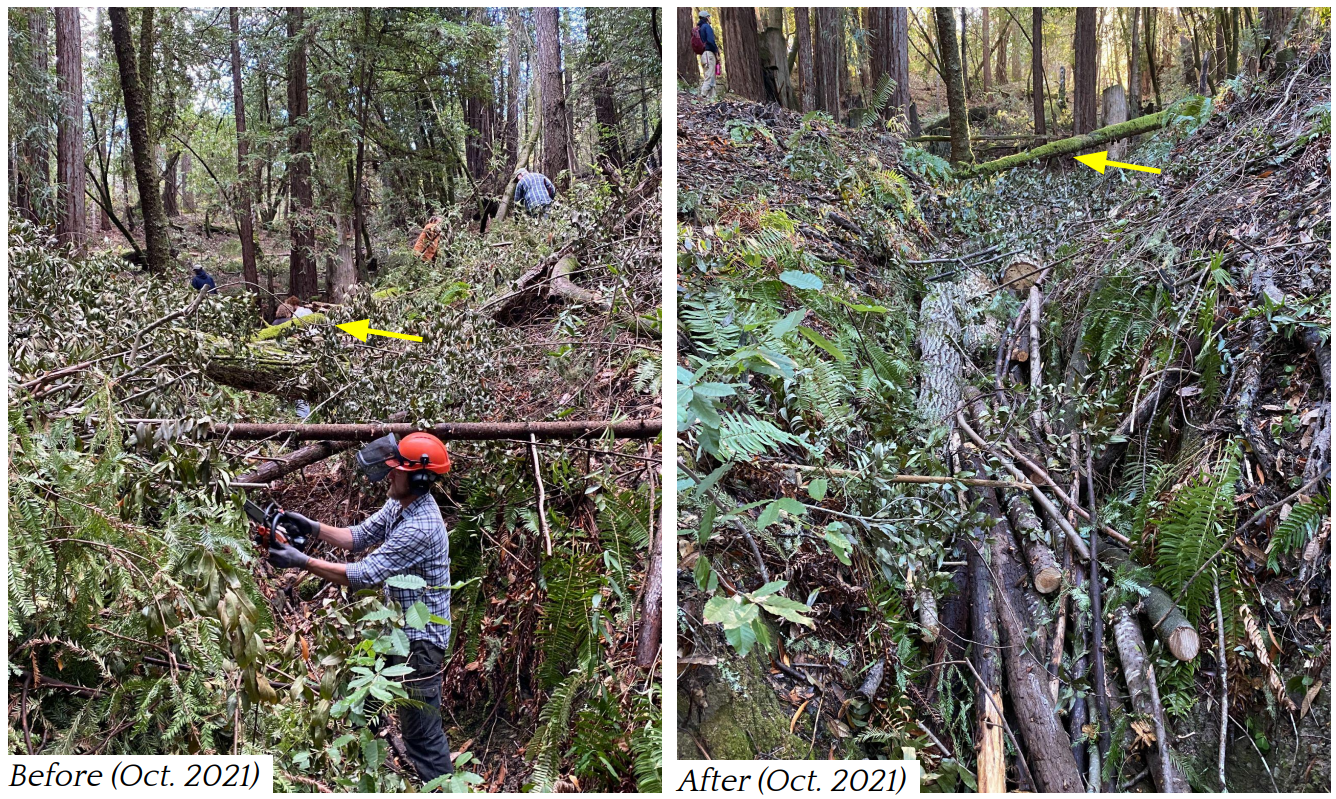
\includegraphics[width=\linewidth]{img/fuels-to-flows2.png}
\end{frame}

\begin{frame}{Expanding the Fuels to Flows program}
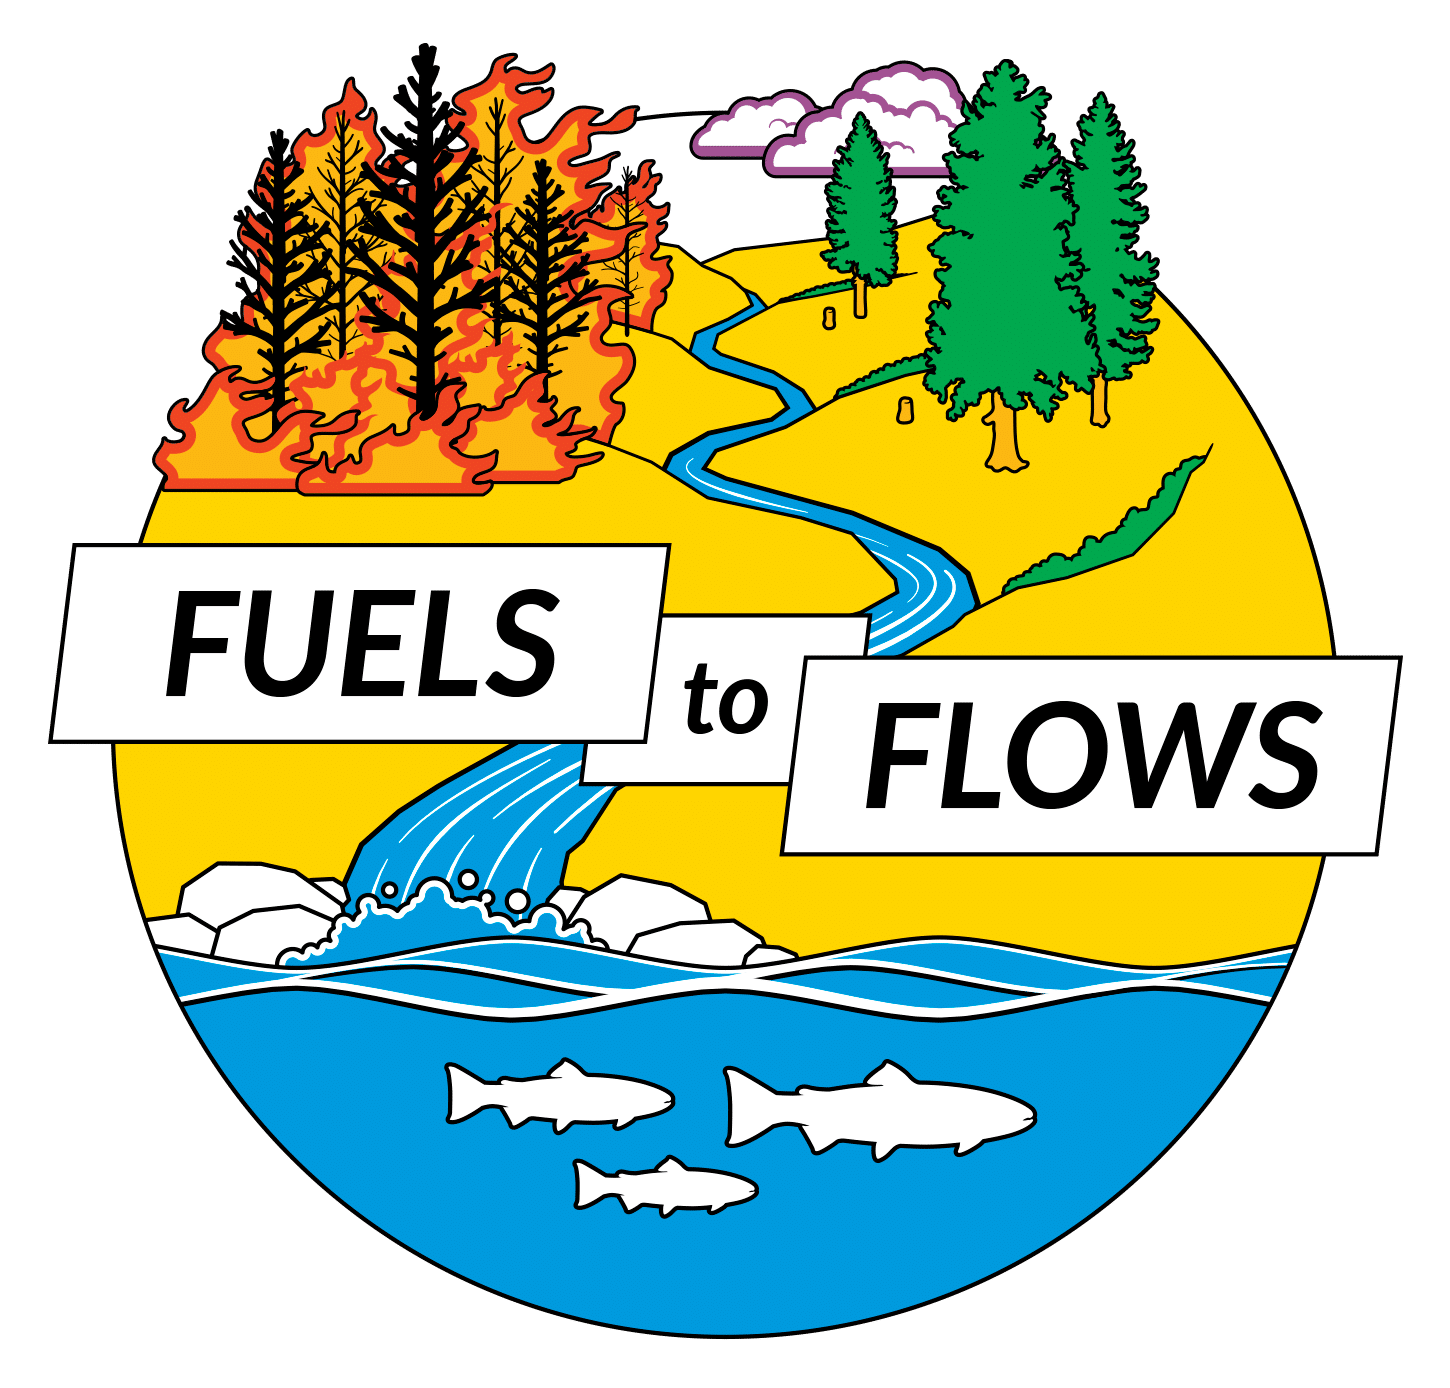
\includegraphics[width=0.1\linewidth]{img/fuels-to-flows-logo.png}
\begin{columns}
\column{0.4\linewidth}
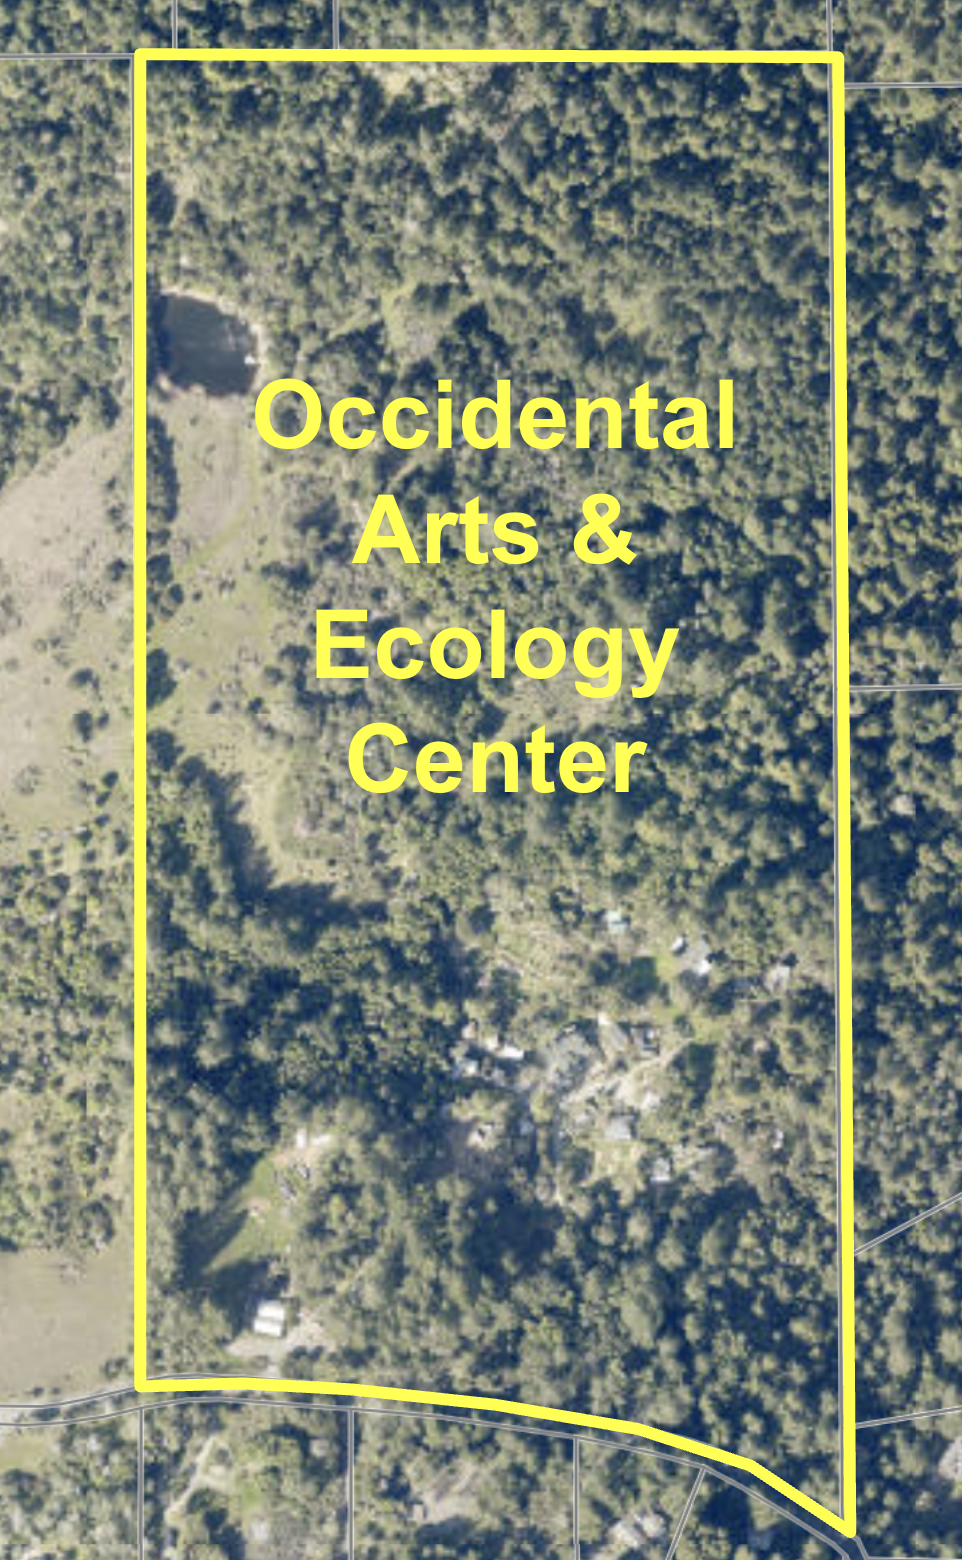
\includegraphics[width=\linewidth]{img/oaec-site.png}
\column{0.6\linewidth}
\begin{itemize}
\item Fuels to Flows has already been implemented at the Occidental Arts \& Ecology Center (OAEC) and Monte Rio National Park.
\item Program Director \textbf{Brock Dolman} was inspired by the use of LIDAR to find lost meadows and proposed a ``found gully'' project to find new sites for Fuels to Flows by air.
\item That's how we at the DSI got involved: we developed a model to find gullies and as well as other tools to discover new Fuels to Flows sites.
\end{itemize}
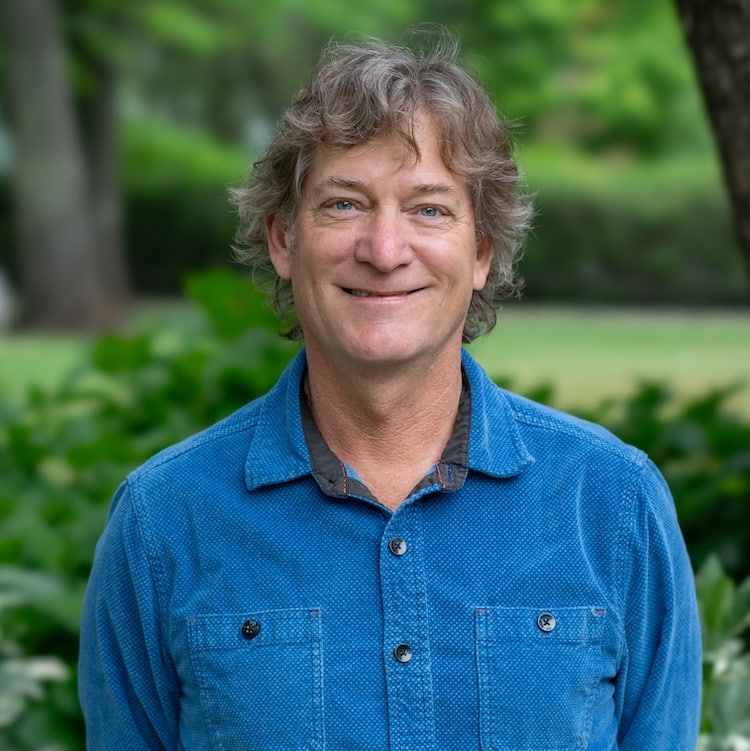
\includegraphics[width=0.3\linewidth]{img/brock.jpg}
\end{columns}
\end{frame}

\begin{frame}
\vfill
\begin{center}
{\Huge Finding gullies}
\end{center}
\vfill
\end{frame}

\begin{frame}{Where are the gullies? --- aerial photography}
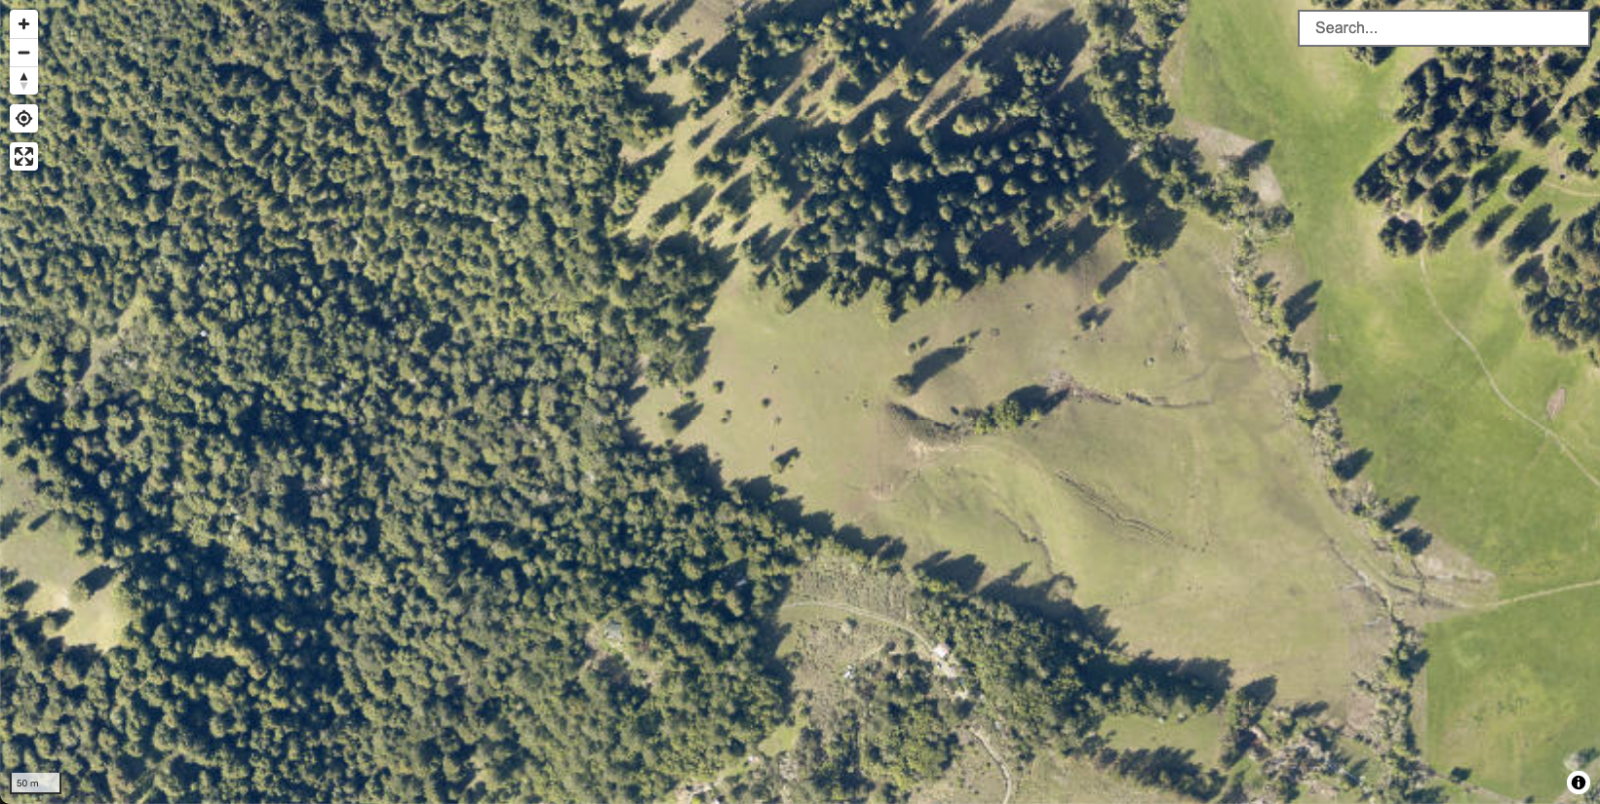
\includegraphics[width=\linewidth]{img/gullies-aerial.png}
\end{frame}

\begin{frame}{Where are the gullies? --- LIDAR hillshade without trees}
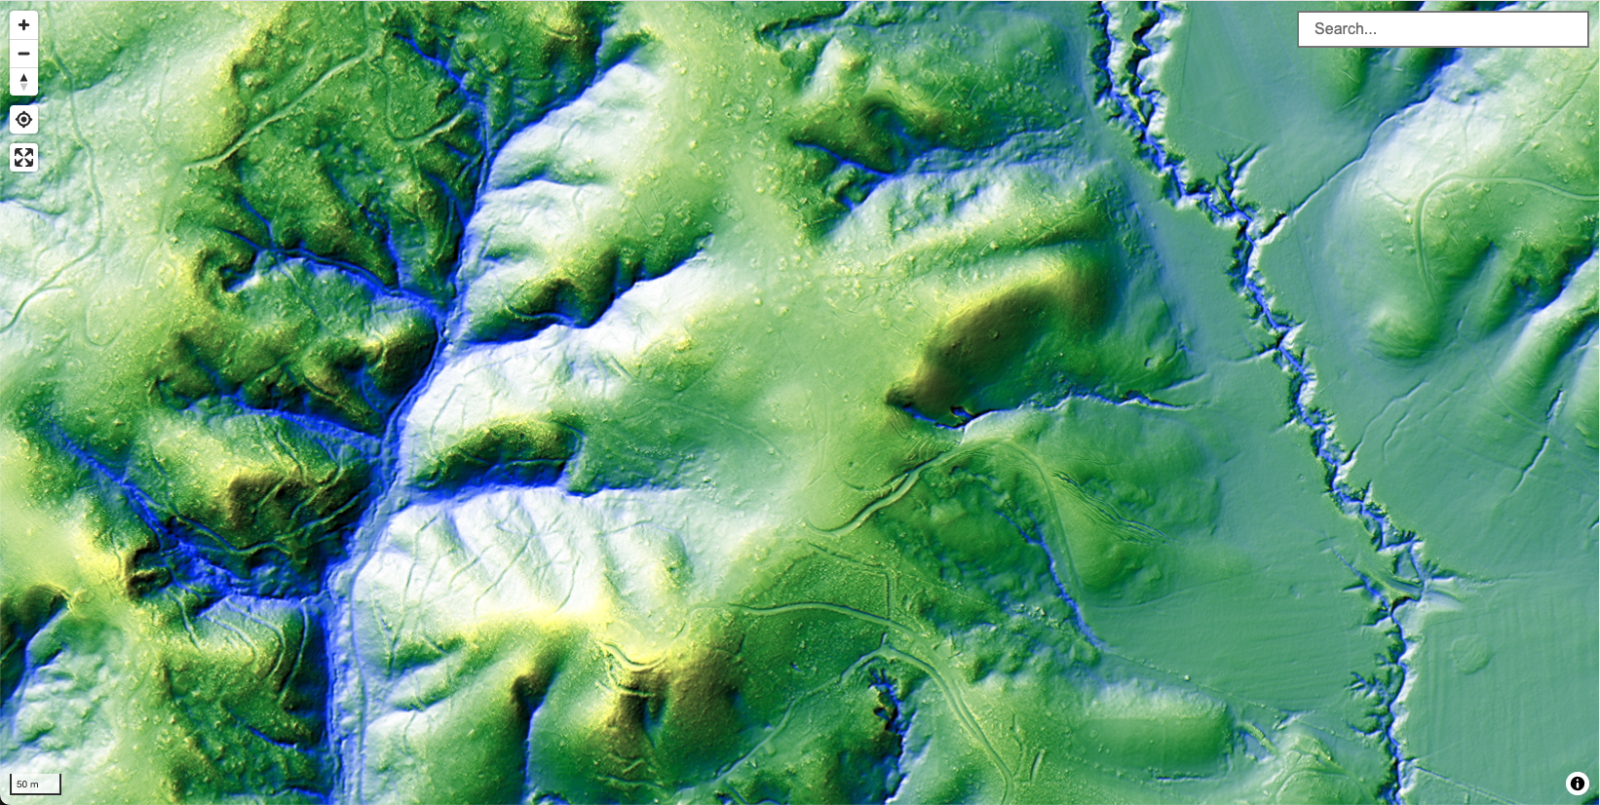
\includegraphics[width=\linewidth]{img/gullies-lidar.png}
\end{frame}

\begin{frame}{Where are the gullies? --- our gully-finding algorithm}
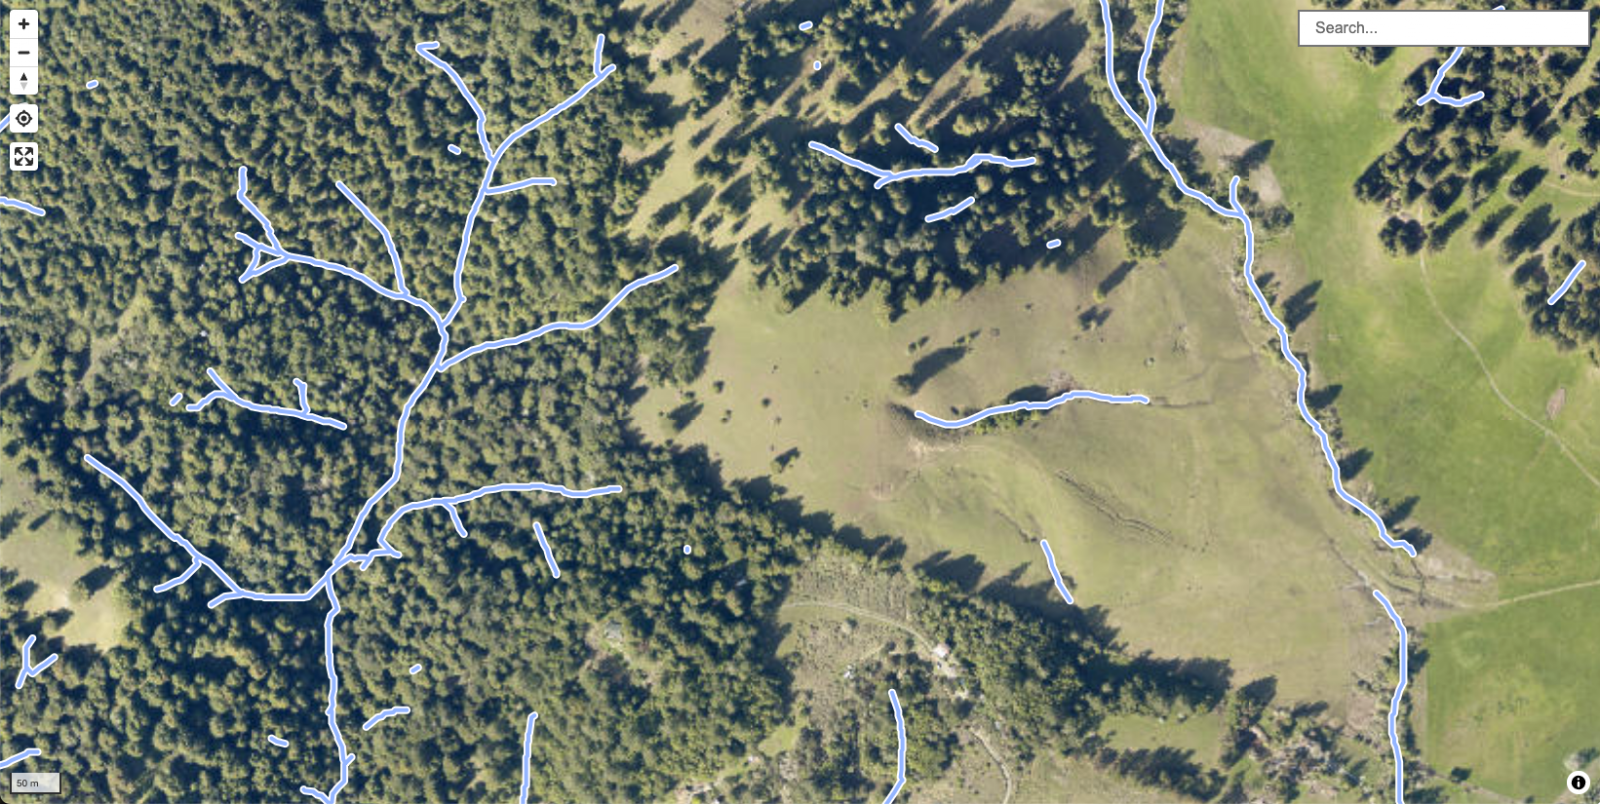
\includegraphics[width=\linewidth]{img/gullies-detected.png}
\end{frame}

\begin{frame}{Publicly available LIDAR for all of Sonoma County, CA}
\begin{columns}
\column{0.4\linewidth}
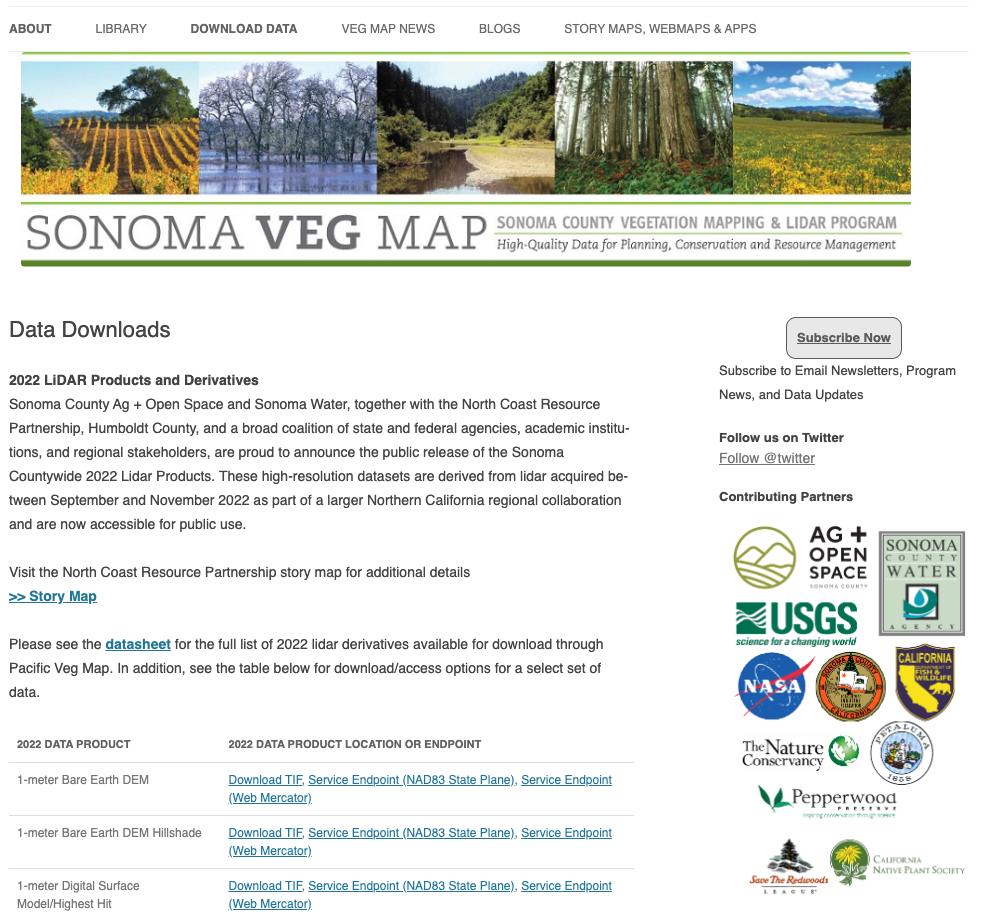
\includegraphics[width=\linewidth]{img/sonomavegmap.png}
\column{0.6\linewidth}
\begin{itemize}
\item Digital Elevation Model (DEM)
\begin{itemize}
\item absolute elevation above sea level
\item in a grid of pixels: $\frac{1}{2}$ meter $\times$ $\frac{1}{2}$ meter
\item complete map in 2013 and 2022
\end{itemize}
\item Ladder fuel proxies
\begin{itemize}
\item (material in 1--4 m) / (material in 0--4 m)
\item (material in 1--8 m) / (material in 0--8 m)
\end{itemize}
\end{itemize}
\end{columns}
\end{frame}

\begin{frame}{Standard technique: difference from mean elevation}
\begin{columns}
\column{0.4\linewidth}
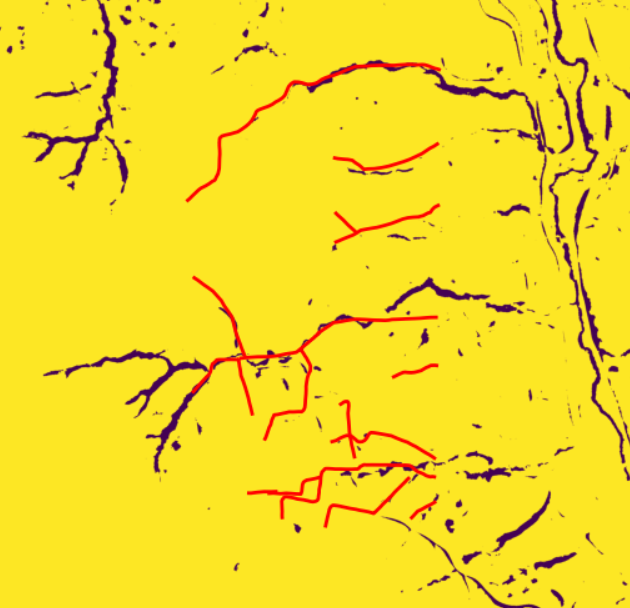
\includegraphics[width=\linewidth]{img/diff-mean-elevation.png}

\textcolor{red}{Red: known gullies on OAEC site}
\column{0.6\linewidth}
\begin{itemize}
\item For example, \href{https://onlinelibrary.wiley.com/doi/epdf/10.1002/esp.1918}{DOI 10.1002/esp.1918}.
\item A gully is an indentation in the ground.
\begin{itemize}
\item Subtract the absolute elevation of each pixel from the average in a 50 meter radius.
\end{itemize}
\item Reliably highlights the locations of known gullies on the OAEC site.
\end{itemize}
\end{columns}
\end{frame}

\begin{frame}{Note that procedure is a convolution!}
Convolution kernel:
\begin{columns}
\column{0.5\linewidth}
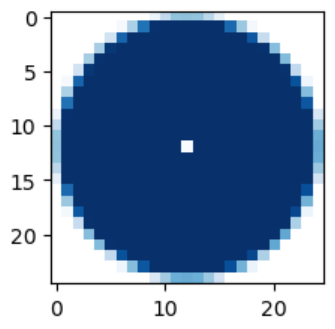
\includegraphics[width=0.7\linewidth]{img/diff-mean-as-kernel.png}

\textcolor{darkorange}{Positive central pixel}

\textcolor{darkorange}{Negative disk}

\textcolor{darkorange}{Sum = 0}
\column{0.5\linewidth}
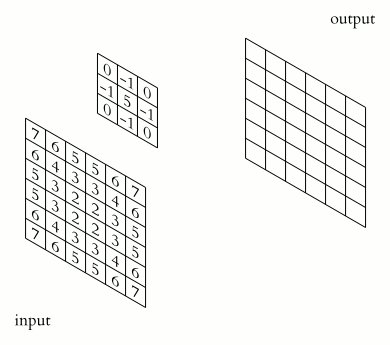
\includegraphics[width=\linewidth]{img/convolution.png}

{\small Convolution animation from Wikipedia}
\end{columns}
\end{frame}

\begin{frame}{What if we used a convolution kernel \textit{shaped} like a gully?}
Convolution kernels:
\begin{columns}
\column{0.4\linewidth}
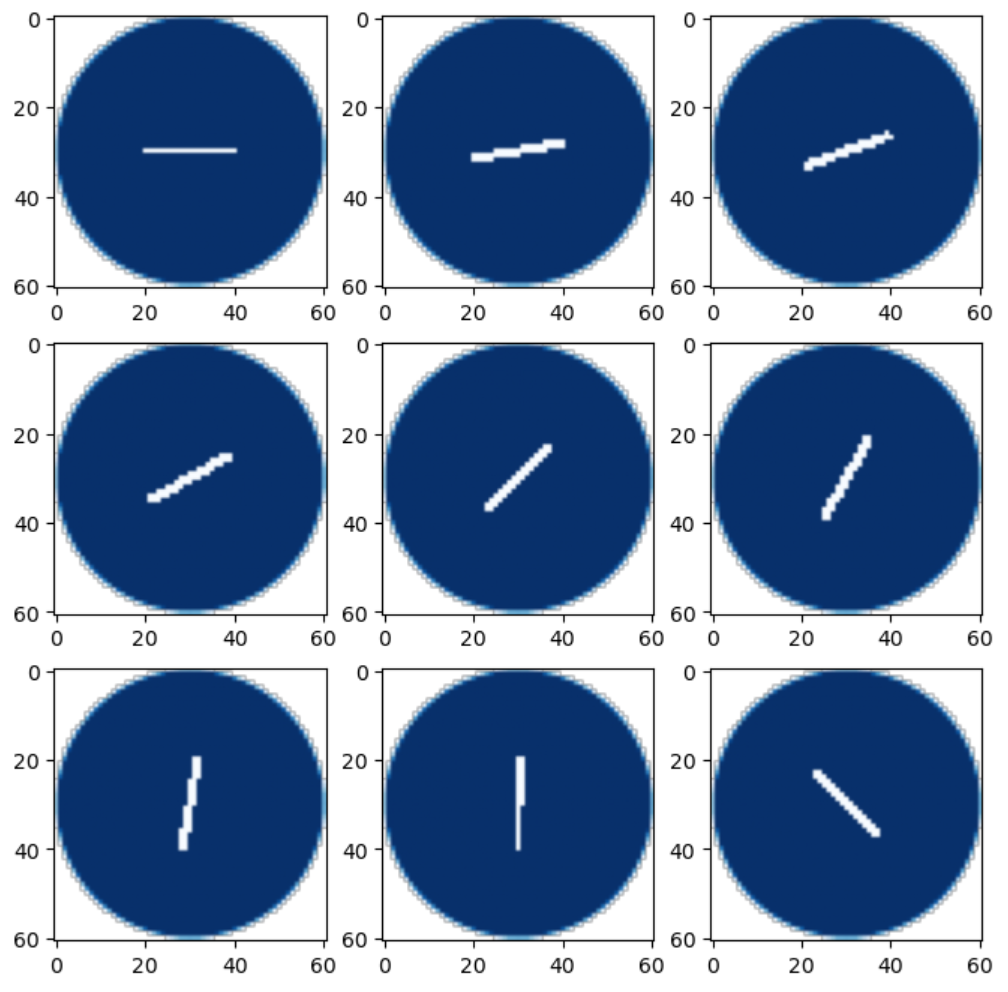
\includegraphics[width=\linewidth]{img/trough-convolutions.png}
\column{0.6\linewidth}
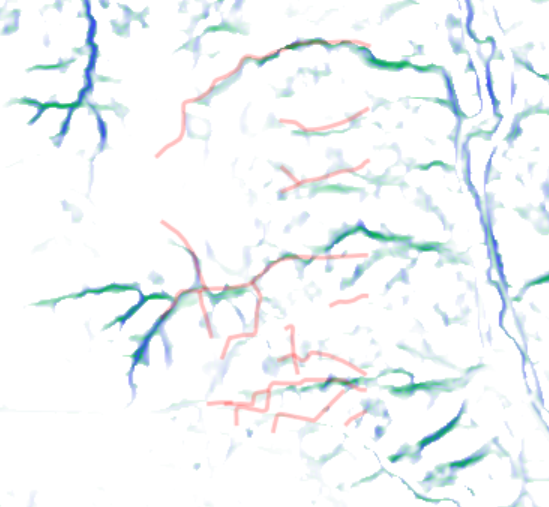
\includegraphics[width=\linewidth]{img/orientation-aware-gullies.png}

\textcolor{red}{Red: known gullies}

\textcolor{darkgreen}{Green: east-west indentation}

\textcolor{darkblue}{Blue: north-south indentation}
\end{columns}
\end{frame}

\begin{frame}{Developing a model}
\begin{itemize}
\item This reasoning ultimately leads to a Convolutional Neural Network (CNN).
\begin{itemize}
\item Rather than building a set of convolution kernels by hand, they'd be learned.
\item As a supervised learning technique, a CNN would require hand-labeled training data.
\end{itemize}
\item We can label some gullies by hand, but not enough to train a CNN.
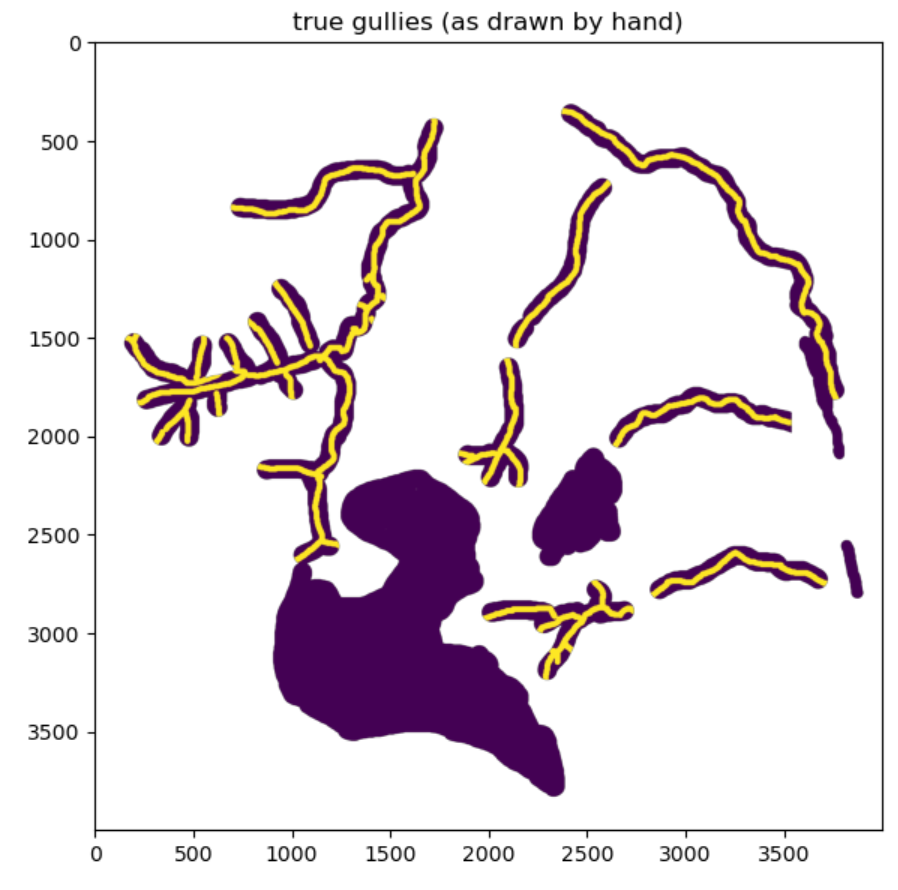
\includegraphics[width=0.3\linewidth]{img/manual-labeling.png}
\item Compromise:
\begin{itemize}
\item We hand-draw gully labels for training data (in-gully, out-of-gully, and unknown) in 9 watersheds.
\item We engineer convolution kernels as features (different segment lengths; anti-cliff veto).
\item Perform logistic regression, which is equivalent to a single CNN layer (with sigmoid activation).
\end{itemize}
\end{itemize}
\end{frame}

\begin{frame}{Gully probability model}
\begin{columns}
\column{0.5\linewidth}
\begin{itemize}
\item Just 7 features
\item Predicts billions of pixels
\item Low correlation among the features:

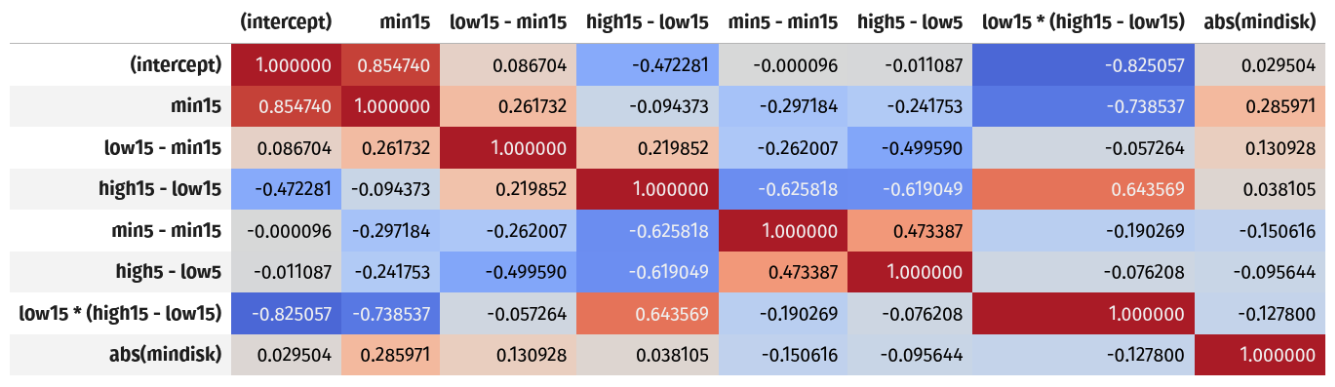
\includegraphics[width=\linewidth]{img/correlation-matrix.png}
\item Minimized loss function $\to$
\end{itemize}
\column{0.5\linewidth}
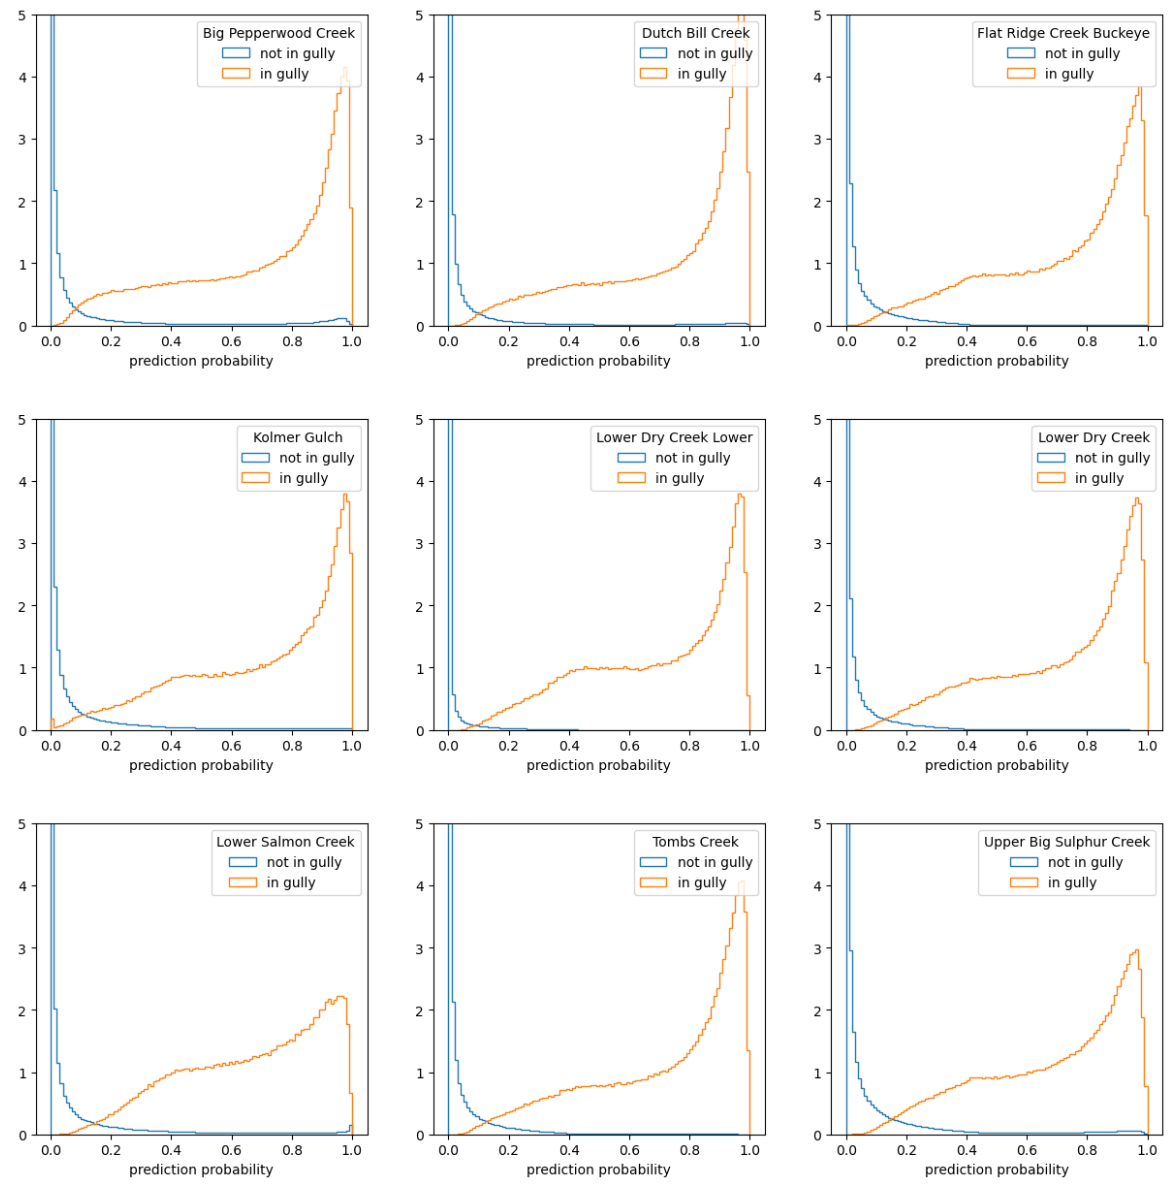
\includegraphics[width=\linewidth]{img/residuals.png}
\end{columns}
\end{frame}

\begin{frame}{Second layer of the ``CNN''}
\begin{itemize}
\item To reduce noise and increase connectivity between real gullies:
\begin{itemize}
\item Pooling: scale gully probability image down by a factor of 2 on each side.
\item Second convolution: use angled kernels again to connect islands.
\end{itemize}
\end{itemize}
\begin{columns}
\column{0.5\linewidth}
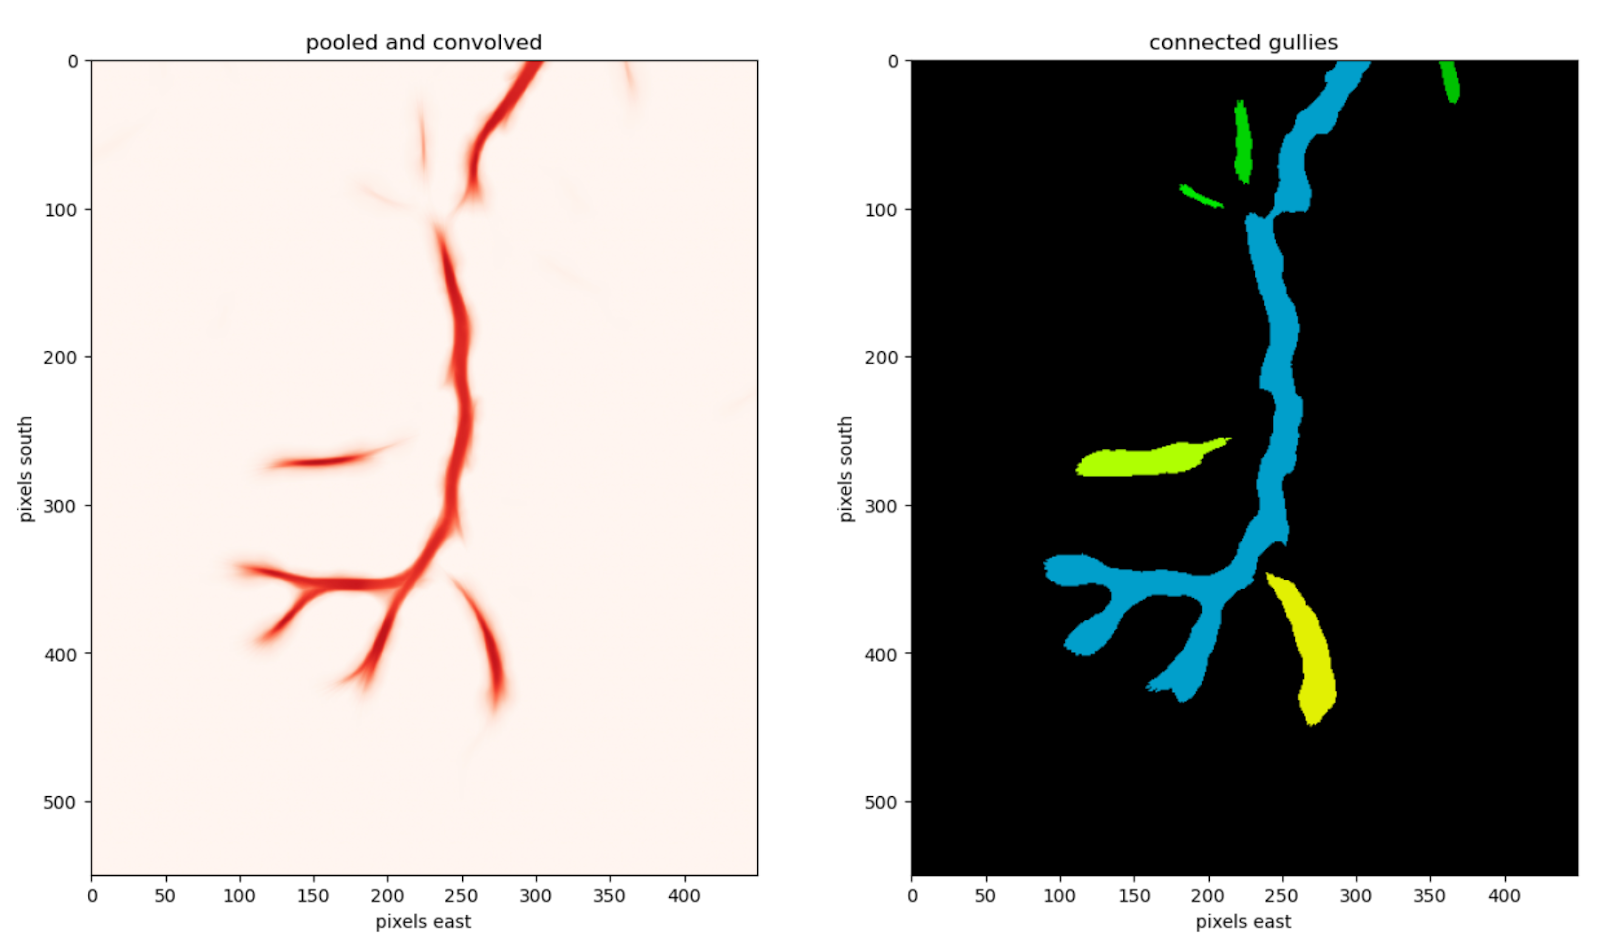
\includegraphics[width=\linewidth]{img/our-model.png}

\begin{center}
Our model
\end{center}
\column{0.5\linewidth}
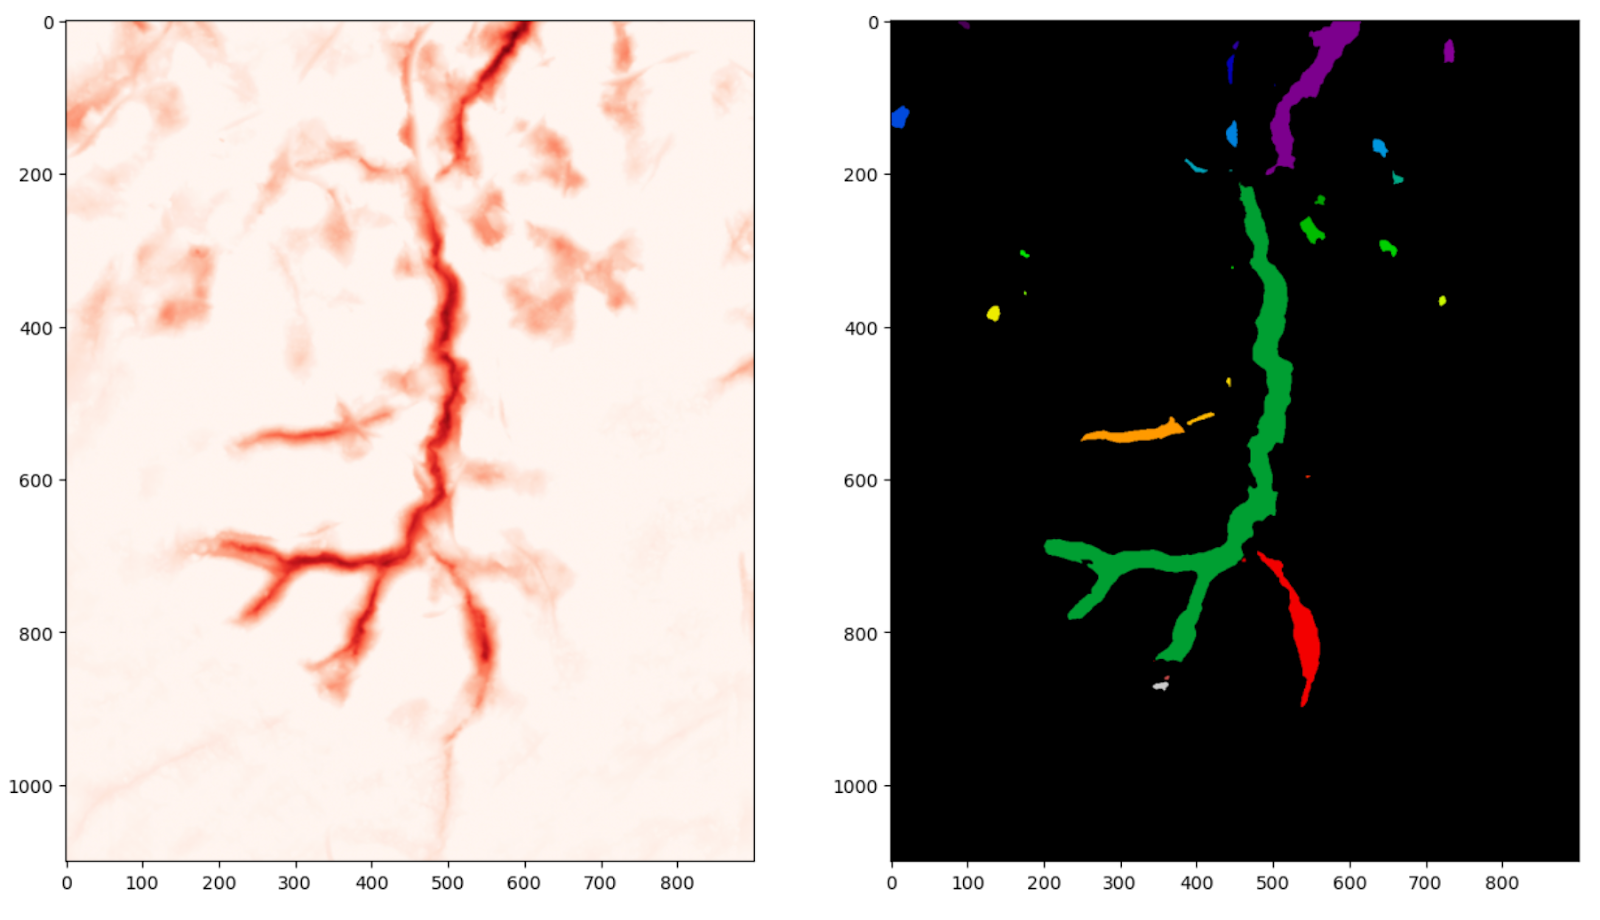
\includegraphics[width=\linewidth]{img/status-quo.png}

\begin{center}
Status quo (diff from mean elevation)
\end{center}
\end{columns}
\end{frame}

\begin{frame}{Final output: a road network/graph}
\begin{columns}
\column{0.5\linewidth}
1. Shrink to centerlines.

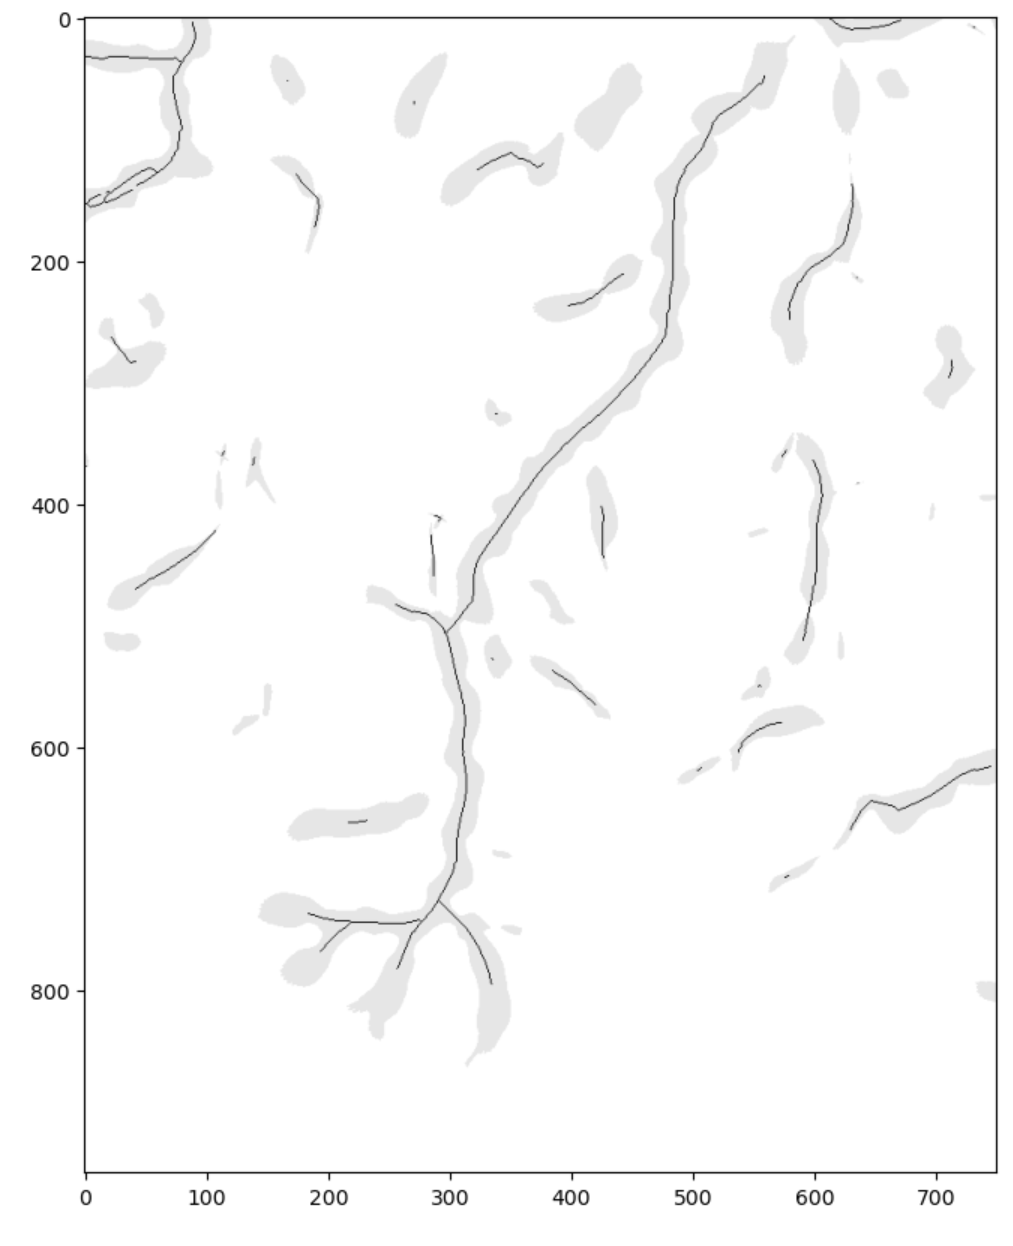
\includegraphics[width=\linewidth]{img/shrink-to-centerlines.png}
\column{0.5\linewidth}
2. Connect segments into a graph.

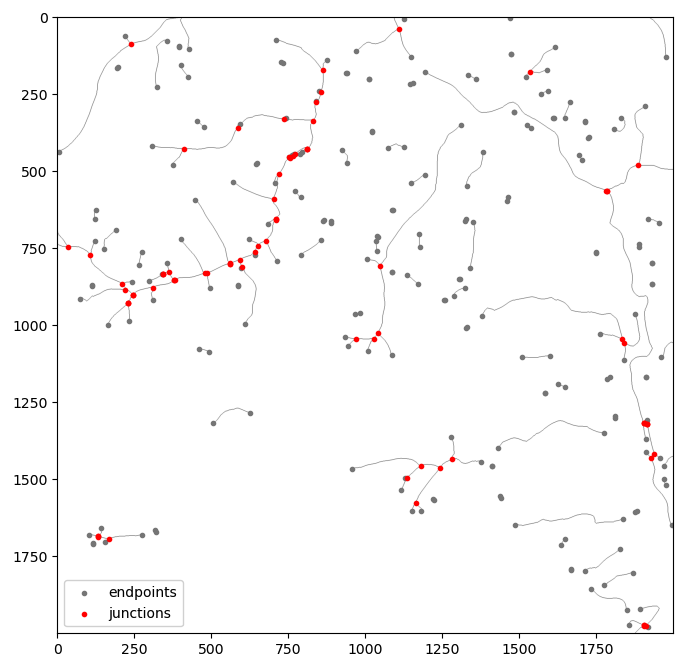
\includegraphics[width=\linewidth]{img/as-a-graph.png}
\end{columns}
\end{frame}

\begin{frame}{Synergy with the DSI Clinic}
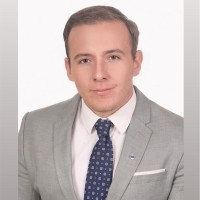
\includegraphics[width=0.2\linewidth]{img/jose-cardona.jpg}
\begin{itemize}
\item Jos\'e Cardona is a masters student in Computational Analysis \& Public Policy who took the DSI Clinic in Fall '25.
\item His project team was analyzing the graph structure of blood vessels in breast cancer MRIs, advised by Anna Woodard and Jim Pivarski (me).
\item He generalized the centerline $\to$ graph algorithm to 3D so that it could be applied to get a 3D graph of blood vessels, rather than a 2D graph of gullies.
\end{itemize}
\begin{columns}
\column{0.5\linewidth}
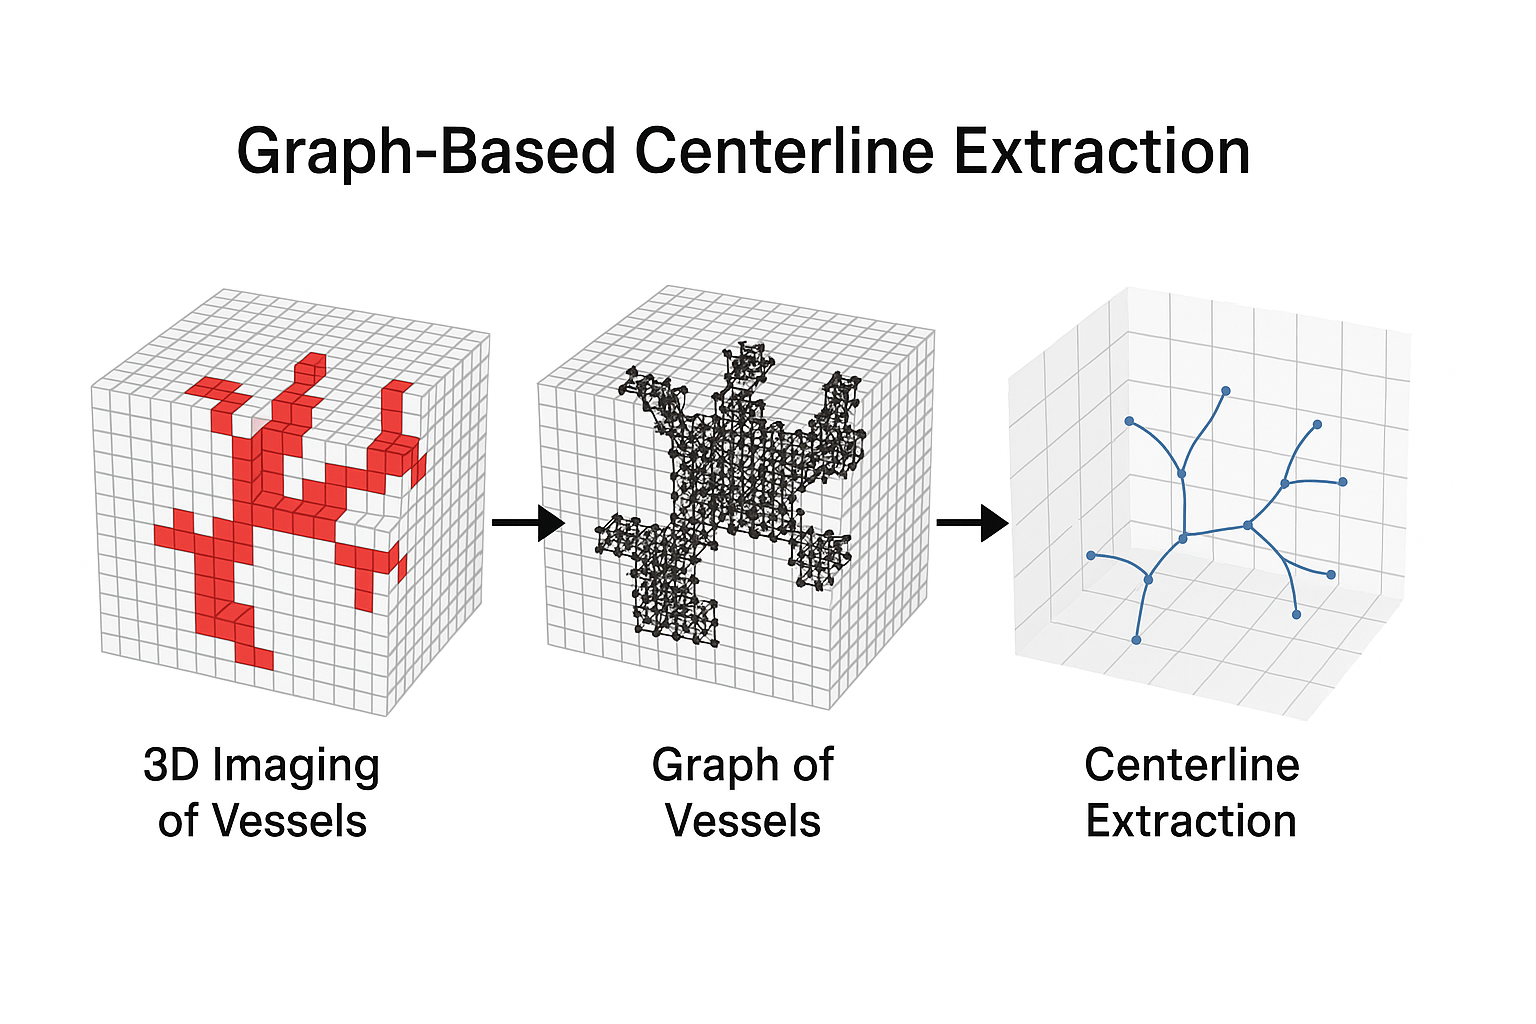
\includegraphics[width=\linewidth]{img/multidim-centerline.png}
\column{0.5\linewidth}
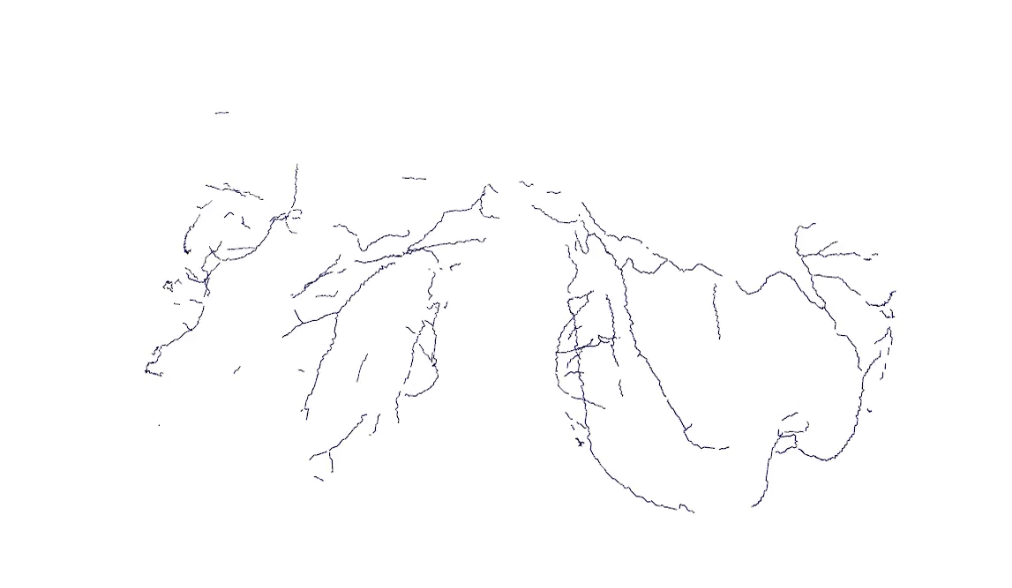
\includegraphics[width=\linewidth]{img/blood-vessels.png}
\end{columns}
\end{frame}

\begin{frame}
\vfill
\begin{center}
{\Huge Delivering results to OAEC}
\end{center}
\vfill
\end{frame}

\begin{frame}{Our final product is a set of map layers}
\begin{itemize}
\item \textcolor{darkorange}{Gully network}
\item \textcolor{darkblue}{2013 and 2021 aerial photography}
\item \textcolor{darkblue}{2013 and 2022 elevation data}
\begin{itemize}
\item \textcolor{darkblue}{Their difference, which measures erosion and deposition}
\end{itemize}
\item \textcolor{darkblue}{Ladder fuel proxies}
\item \textcolor{darkgrey}{Land ownership boundaries and addresses (to contact landowners)}
\end{itemize}

\vspace{0.5 cm}
We made \href{https://github.com/dsi-clinic/oaec-found-gully?tab=readme-ov-file\#data-products}{a folder of data files} available for GIS experts, but

\begin{itemize}
\item not all users are likely to be experts;
\item some of these files are huge (up to 150 GB).
\end{itemize}
\end{frame}

\begin{frame}{Instead, we built a specialized map webapp}
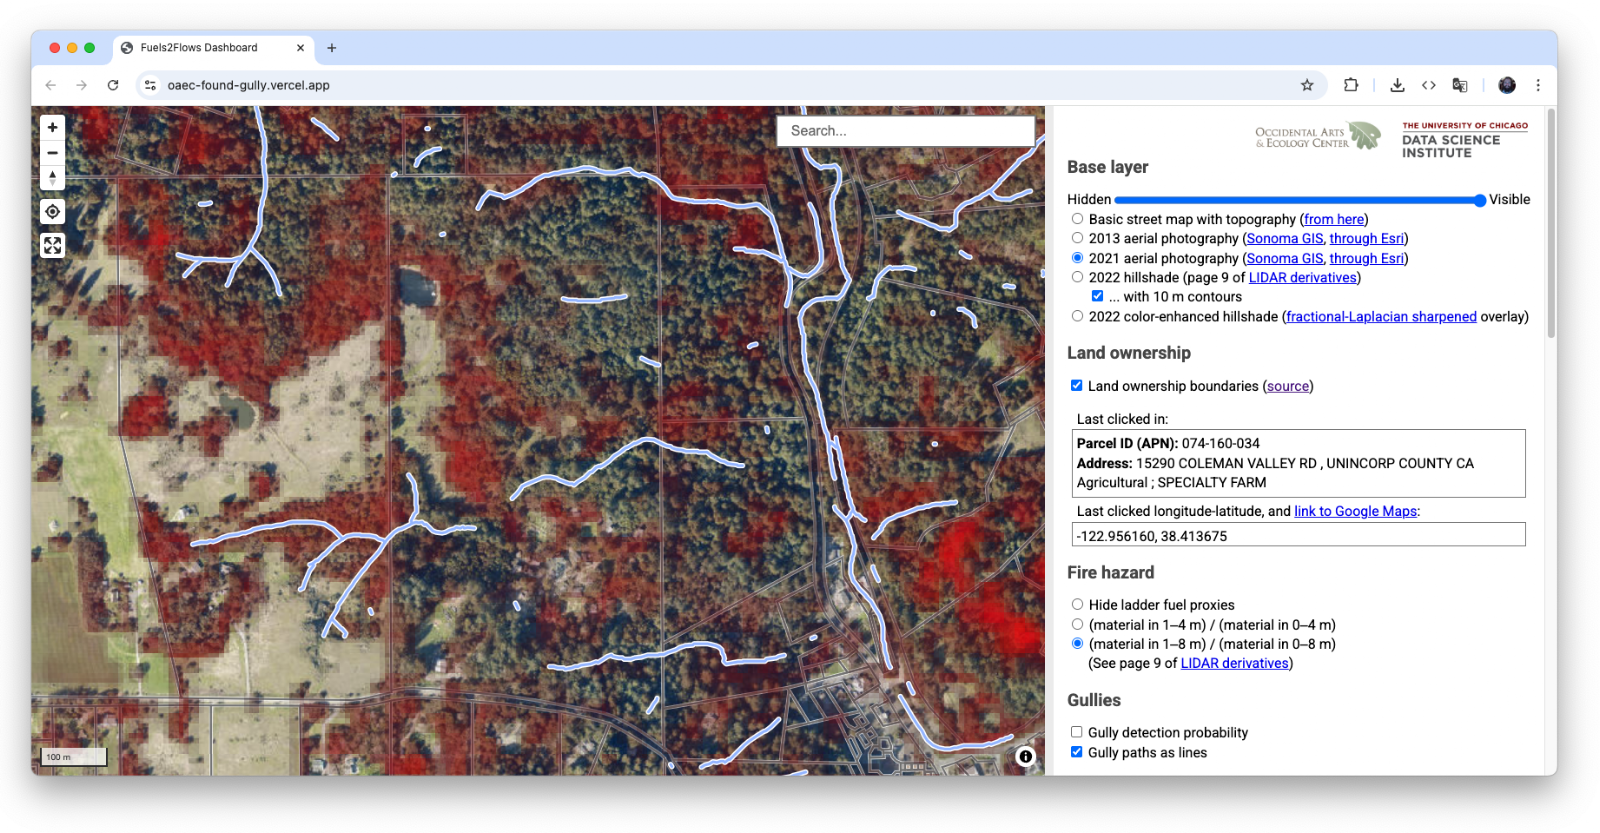
\includegraphics[width=\linewidth]{img/webapp.png}
\end{frame}

\begin{frame}
\vfill
\begin{center}
{\Huge switch to \href{https://oaec-found-gully.vercel.app/}{live demo}}
\end{center}
\vfill
\end{frame}

\begin{frame}{Technical highlight}
\begin{columns}
\column{0.6\linewidth}
\begin{itemize}
\item For performance, the visible layers are delivered on demand as tiles.
\item No server required: the PMTiles file format is addressable one tile at a time.
\item The ``volume of erosion'' and ``elevation along line'' features also use PMTiles to download elevation data one tile at a time.
\begin{itemize}
\item But elevation data needs float32 precision, and PMTiles must be RGBA images.
\item So we bit-cast the four 8-bit channels as a 32-bit float.
\item The (unshown) images look like this:
\end{itemize}
\end{itemize}
\column{0.4\linewidth}
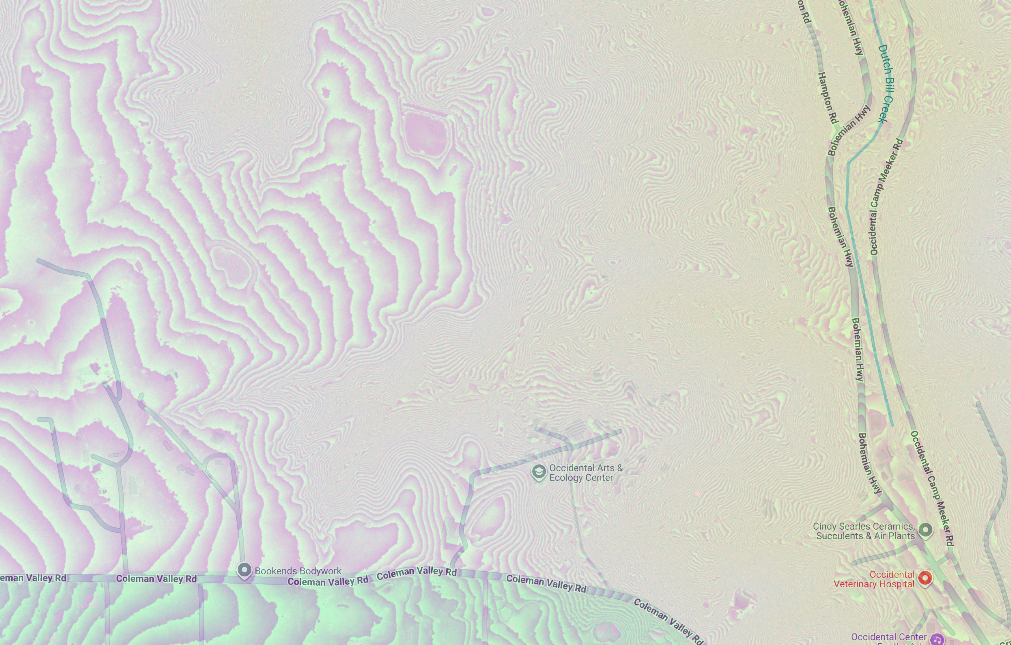
\includegraphics[width=\linewidth]{img/pmtiles-bitcast.png}
\end{columns}
\end{frame}

\begin{frame}
\vfill
\begin{center}
{\Huge Impact}
\end{center}
\vfill
\end{frame}

\begin{frame}{This system is for assessing new sites for Fuels to Flows}
\begin{itemize}
\item We rely, in part, on Brock's network of agencies and landowners who might apply Fuels to Flows on their sites.
\item He has been spreading awareness of our site among his contacts.
\item We've had two interesting Zoom calls:
\begin{itemize}
\item Adam Cummings at \href{https://www.thewatershedcenter.com/}{the Watershed Center}
\item Matt O'Connor and Jeremy Koor at \href{https://www.oe-i.com/}{O'Connor Environmental, Inc.}
\end{itemize}
\item and one known user:
\begin{itemize}
\item Fatima Burhan at \href{https://sonomarcd.org/}{Sonoma Resource Conservation District}
\end{itemize}
\item The gully map is technically complete, but the networking has just begun!
\end{itemize}
\end{frame}

\begin{frame}
\vfill
\begin{center}
{\Huge Questions?}
\end{center}
\vfill
\end{frame}

\end{document}
